% +++++++++++++++++++++++++++++++++++++++++++++++++++++++++++
% University of Southern Maine
% Department of Computer Science
% Discrete Mathematics II (COS 280)
% James Quinlan (https://cs.usm.maine.edu/~james.quinlan/)
% Homework Template
% +++++++++++++++++++++++++++++++++++++++++++++++++++++++++++


% EDIT Lines: 11, 12, 13
\def\filename{Genetic Algorithm}   		   % included file (edit file)
\def\chapsec{Chapter 10}  % Chapter/Section/Topic
\def\yourname{Genetic Algorithm and Genetic Programming} % Your name
\def\course{COS 485}		   % Course (if different)



% ---------------- Do NOT Edit Below ------------------------
% -----------------------------------------------------------
\documentclass[11pt]{article}

\def\pf{\textit{Proof}: }

\usepackage{mathtools}
\usepackage{epsfig}
\usepackage{amsfonts}
\usepackage{amssymb}
\usepackage{amstext}
\usepackage{amscd}
\usepackage{amsmath}
\usepackage{xspace}
\usepackage{theorem}
\usepackage{float}
\usepackage[table]{xcolor}
\usepackage{color}
\usepackage{soul}
\usepackage{booktabs}
\usepackage{outlines}
\usepackage{enumitem}
\usepackage{algorithm}
\usepackage{algpseudocode}
\usepackage{pgf-pie}
\setenumerate[1]{label=\arabic*.}
\setenumerate[2]{label=(\alph*).}
\setenumerate[3]{label=\roman*.}
\setenumerate[4]{label=\alph*.}

\usepackage{hyperref}
\hypersetup{
    colorlinks=true,
    linkcolor=blue,
    filecolor=magenta,      
    urlcolor=cyan,
    pdftitle={\filename},
    pdfpagemode=FullScreen,
    }

% TikZ
\usepackage{tikz}
\usepackage{pgfplots}
\pgfplotsset{compat=1.15}
\usepackage{mathrsfs}
\usetikzlibrary{arrows}

% Colors
\definecolor{stainlessSteel}{cmyk}{0,0,0.02,0.12}

% Document Geometry
\makeatletter
 \setlength{\textwidth}{6.75in}
 \setlength{\oddsidemargin}{0in}
 \setlength{\evensidemargin}{0in}
 \setlength{\topmargin}{0.0125in}
 \setlength{\textheight}{9.0in}
 \setlength{\headheight}{0pt}
 \setlength{\headsep}{0pt}
 \setlength{\marginparwidth}{59pt}

 \setlength{\parindent}{0pt}
 \setlength{\parskip}{5pt plus 1pt}
 \setlength{\theorempreskipamount}{5pt plus 1pt}
 \setlength{\theorempostskipamount}{0pt}
 \setlength{\abovedisplayskip}{8pt plus 3pt minus 6pt}
 \setlength{\intextsep}{15pt plus 3pt minus 6pt}

 % Headings
 \renewcommand{\section}{\@startsection{section}{1}{0mm}%
    {2ex plus -1ex minus -.2ex}%
    {1.3ex plus .2ex}%
    {\normalfont\Large\bfseries}}%
 \renewcommand{\subsection}{\@startsection{subsection}{2}{0mm}%
    {1ex plus -1ex minus -.2ex}%
    {1ex plus .2ex}%
    {\normalfont\large\bfseries}}%
 \renewcommand{\subsubsection}{\@startsection{subsubsection}{3}{0mm}%
    {1ex plus -1ex minus -.2ex}%
    {1ex plus .2ex}%
    {\normalfont\normalsize\bfseries}}
 \renewcommand\paragraph{\@startsection{paragraph}{4}{0mm}%
    {1ex \@plus1ex \@minus.2ex}%
    {-1em}%
    {\normalfont\normalsize\bfseries}}
 \renewcommand\subparagraph{\@startsection{subparagraph}{5}{\parindent}%
    {2.0ex \@plus1ex \@minus .2ex}%
    {-1em}%
    {\normalfont\normalsize\bfseries}}
\makeatother

\newcounter{thelecture}

\newenvironment{proof}{{\bf Proof:  }}{\hfill\rule{2mm}{2mm}}
\newenvironment{proofof}[1]{{\bf Proof of #1:  }}{\hfill\rule{2mm}{2mm}}
\newenvironment{proofofnobox}[1]{{\bf#1:  }}{}
\newenvironment{example}{{\bf Example: }}{\hfill\rule{0mm}{0mm}} % change 2mm 2mm for square

%\renewcommand{\theequation}{\thesection.\arabic{equation}}
%\renewcommand{\thefigure}{\thesection.\arabic{figure}}

\newtheorem{fact}{Fact}
\newtheorem{lemma}[fact]{Lemma}
\newtheorem{theorem}[fact]{Theorem}
\newtheorem{definition}[fact]{Definition}
\newtheorem{corollary}[fact]{Corollary}
\newtheorem{proposition}[fact]{Proposition}
\newtheorem{claim}[fact]{Claim}
\newtheorem{exercise}[fact]{Exercise}

% math notation
\newcommand{\R}{\ensuremath{\mathbb R}}
\newcommand{\Z}{\ensuremath{\mathbb Z}}
\newcommand{\N}{\ensuremath{\mathbb N}}
\newcommand{\B}{\ensuremath{\mathbb B}}
\newcommand{\F}{\ensuremath{\mathcal F}}
\newcommand{\SymGrp}{\ensuremath{\mathfrak S}}
\newcommand{\prob}[1]{\ensuremath{\text{{\bf Pr}$\left[#1\right]$}}}
\newcommand{\expct}[1]{\ensuremath{\text{{\bf E}$\left[#1\right]$}}}
\newcommand{\size}[1]{\ensuremath{\left|#1\right|}}
\newcommand{\ceil}[1]{\ensuremath{\left\lceil#1\right\rceil}}
\newcommand{\floor}[1]{\ensuremath{\left\lfloor#1\right\rfloor}}
\newcommand{\ang}[1]{\ensuremath{\langle{#1}\rangle}}
\newcommand{\poly}{\operatorname{poly}}
\newcommand{\polylog}{\operatorname{polylog}}

% Anupam's abbreviations
\newcommand{\e}{\epsilon}
\newcommand{\half}{\ensuremath{\frac{1}{2}}}
\newcommand{\junk}[1]{}
\newcommand{\sse}{\subseteq}
\newcommand{\union}{\cup}
\newcommand{\meet}{\wedge}
\newcommand{\dist}[1]{\|{#1}\|_{\text{dist}}}
\newcommand{\hooklongrightarrow}{\lhook\joinrel\longrightarrow}
\newcommand{\embeds}[1]{\;\lhook\joinrel\xrightarrow{#1}\;}
\newcommand{\mnote}[1]{\normalmarginpar \marginpar{\tiny #1}}

% -----------------------------------------------------------
% Header
\newcommand{\hwheadings}[3]{
{\chapsec } \hfill {{ \yourname }} \hfill {{ \course #1}}\\
{{\bf } #2} \hfill { #3} 
\rule[0.051in]{\textwidth}{0.0025in}
%\thispagestyle{empty}
}

% Document begins here 
\begin{document}
\hwheadings{}{}{}
\section*{\centering Genetic Algorithms and Genetic Programming}

\section*{Overview}
\label{sec:overview}

\begin{outline}[enumerate]
  \1 Genetics Review 
  \1 General Genetic Algorithm 
  \1 Implementation Examples 
\end{outline}

\section*{Genetics Review}%
\label{sec:review}

An \textit{`organism'} or \textit{`individual'} is a form of life such as a plant or animal.
Chromosomes carry biological information or characteristics of an individual.
During reproduction, there is several things that happen to form the child individuals.
There is a \textit{`crossing over'} where genetic material is exchanged and there is a small, random
chance of a mutation. \textit{`Natual selection'} is the process by which organisms with traits
that are better suited to their environment reproduce in higher numbers, increasing the prescense of those
traits.

In a Genetic Algorithm (GA), \textit{`individuals'} are canidate solutions. Each
solution has \textit{`chromosomes'} or a unique identifier that represents its 
corresponding canidate solution. \textit{`Natural selection'} occurs through a 
fitness function that determines the overall fitness of the canidate solution.
\textit{`Crossing over'} happens by exchanging information between the identifier for the solution.
\textit{`Mutations'} happen by a bitflip, or some other change to the information representing a solution.

\section*{General Genetic Algorithm}%
\label{sec:general-algorithm}

\begin{algorithm}
  \label{alg:genetic}
  \caption{Generic Genetic Algorithm}\label{alg:cap}
  \begin{algorithmic}
    \State $i = 0$ \Comment{Generation counter}
    \State initialize population $P_{0}$ \Comment{Decide on sample size; $n$}
    \Repeat
    \State Evaluate fitness of each indivitual in population $P_{i}$ ; \Comment{Fitness function, $f(x_{i})$}
    \State Select individuals for reproduction based on fitness ; 
      \State Perform crossover and mutation on the selected individuals ;
      \State $i++$;
      \Until{terminal condition is met ;} \Comment{A certain number of generations or average fitness}
  \end{algorithmic}
\end{algorithm}

The probability of selecting a sample, $x_{i}$ for reproduction, with 
$n$ being the sample size, is defined by:

\[
  P(x_{i}) = \frac{f(x_{i})}{\sum_{j=1}^{n} f(x_{j})}
\]
\section*{Implementation Example}%
\label{sec:example}

Suppose we have this \textit{fitness function} and the goal is to \textit{maximize} it.

\[
  f(x) = \sin\left(\frac{x\pi}{256}\right) \textrm{ with the interval } 0 \le x \le 255 \textrm{ \& } x \in \Z
.\] 

We can represent canidate solutions with 8 bits; a byte. Since the goal is to maximize this function,
and the values are locked between $0 - 1$, we will just use the value of the function to represent fitness for 
a canidate solution.

The first step is to select a population size, which will be 8.
Then, to randomly select individuals from the population, we will generate random numbers
in our interval, $0-255$.

\begin{table}[H]
  \centering
  \caption{Normed Fitness\\}
  \label{tab:fitness}

  \begin{tabular}{|| c | c | c | c | c ||}
    \hline 
    $x$ & Representation & $f(x)$ & Normed $f(x)$ & Cumulative $f(x)$ \\
    \hline \hline
    189 & 1 0 1 1 1 1 0 1 & .733 & .144 & .144 \\
    \hline
    216 & 1 1 0 1 1 0 0 0 & .471 & .093 & .237 \\
    \hline
    99 & 0 1 1 0 0 0 1 1 & .937 & .184 & .421 \\
    \hline
    236 & 1 1 1 0 1 1 0 0 & .243 & .048 & .469 \\
    \hline
    174 & 1 0 1 0 1 1 1 0 & .845 & .166 & .635 \\
    \hline
    74 & 0 0 1 0 0 0 1 1 & .788 & .155 & .790 \\
    \hline
    35 & 0 0 1 0 0 0 1 1 & .416 & .082 & .872 \\
    \hline
    53 & 0 0 1 1 0 1 0 1 & .650 & .128 & 1.000 \\
    \hline 
  \end{tabular}
\end{table}

To start selecting samples, find each sample's \textit{Cumulative Normed Fitness}
which will allow for selection using a random number generator between 0-1. The \textit{Cumulative Normed Fitness}
should always add up to 1.0, after normalizing fitness.

\[
  \sum_{i=1}^{n} P(x_{i}) = 1.0
\] 

\begin{center}
  \centering{Probability of selection using Cumulative Norm} \\
  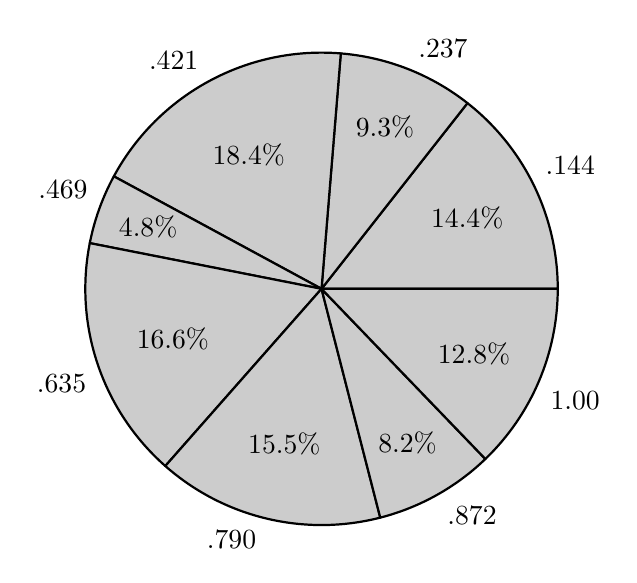
\begin{tikzpicture}
    \label{fig:probability}
    \pie[color={black!20}]
    {14.4/.144, 9.3/.237, 18.4/.421, 4.8/.469, 16.6/.635, 15.5/.790, 8.2/.872, 12.8/1.00}
  \end{tikzpicture}
\end{center}

To select an individual, generate a random number between $0 - 1$. Then find the two numbers
that surround your selection. The individual who is being represented by the larger of the two
is selected for reproduction.

\begin{table}[H]
  \centering
  \caption{Parent-Child Crossover Table}
  \label{tab:Parent-Child Crossover Table}

    \begin{tabular}{||c | c | c||}
    \hline
    Selected Numbers & Parent & Children \\
    \hline \hline
    $3 \cdots 6$ & 0 1 1 $\|$ \textbf{0 0 0} $\|$  1 1 & 0 1 1 $\|$ \textbf{ 1 0 1 } $\|$ 1 1 \\
    $3 \cdots 6$ & 0 0 1 $\|$\textbf{ 1 0 1} $\|$  0 1 & 0 0 1 $\|$ \textbf{ 0 0 0 } $\|$ 0 1 \\
    \hline
    $1 \cdots 5$ & 1 $\|$ \textbf{0 1 0 1} $\|$ 0 0 1 & 1 $\|$  \textbf{1 1 1 0} $\|$ 0 0 1 \\
    $1 \cdots 5$ & 0 $\|$ \textbf{1 1 1 0} $\|$ 1 0 1 & 0 $\|$  \textbf{0 1 0 1} $\|$ 1 0 1 \\
    \hline
  \end{tabular}
\end{table}

In this example, two random numbers between zero and the bitsize are chosen, and the two parents
exchange the bits between the two selected points.


\begin{table}[H]
  \centering
  \caption{Mutation Table}
  \label{tab:Mutation Table}

  \begin{tabular}{||c | c | c||}
    \hline
    Individual & Mutation & New $x$ \\
    \hline \hline
    0 1 1 \textbf{1} 0 1 1 1 & 0 1 1 \textbf{0} 0 1 1 1 & 103\\
    \hline
    0 0 1 0 0 0 0 1 & 0 0 1 0 0 0 0 1 & 33\\
    \hline
    1 1 1 1 0 0 0 \textbf{1} & 1 1 1 1 0 0 0 \textbf{0} & 240\\
    \hline
    0 \textbf{0} 1 0 1 1 0 1 & 0 \textbf{1} 1 0 1 1 0 1 & 109 \\
    \hline
  \end{tabular}
\end{table}

Each individual has a very low percentage to mutate. For this example, a bit flip
will be used as a mutation. After mutation occurs, the newly generated individuals are the `next generation'
and the reproduction process starts again.

\end{document}
% -----------------------------------------------------------
